\documentclass{beamer}
% Setup appearance:
\usepackage{lmodern}
\usepackage[labelformat=empty,font=scriptsize,skip=0pt,justification=justified,singlelinecheck=false]{caption}
\setbeamertemplate{footline}[frame number]

 
%encoding
%--------------------------------------
\usepackage[utf8]{inputenc}
\usepackage[T1]{fontenc}
%--------------------------------------
 
%Portuguese-specific commands
%--------------------------------------
\usepackage[portuguese]{babel}
%--------------------------------------
 
%Hyphenation rules
%--------------------------------------
\usepackage{hyphenat}
\hyphenation{mate-mática recu-perar}


%remove the icon
\setbeamertemplate{bibliography item}{}

%remove line breaks
\setbeamertemplate{bibliography entry title}{}
\setbeamertemplate{bibliography entry location}{}
\setbeamertemplate{bibliography entry note}{}



\title[Artigo]{Antecipação e adaptação: como incorporar os dinamismos do mundo financeiro}
\author[Igor Nascimento]{Igor Nascimento}
\institute[LAMFO]{Laboratório de Aprendizado de Máquina em Finanças e Organizações - LAMFO}
\date[2018]{28/02/2018}

\begin{document}

\begin{frame}
  \titlepage
\end{frame}

\section{Introdução}

\begin{frame}{Visão geral}


\vspace{.15cm}
\begin{enumerate}
\item Contexto
\vspace{.15cm}
\item Amostragem aleatória
\vspace{.15cm}
\item Modelos Dinâmicos
\vspace{.15cm}
\item Filtro de Partículas
\end{enumerate}

\end{frame}



\begin{frame}{Mundo financeiro}

O investidor (banco, pessoa física, fundo de investimento, fundo de pensão) possui um capital e deseja utiliza-lo para atingir um objetivo:

\begin{itemize}
\item Rendimento superior a taxa de captação 
\item Segurança financeira
\item Lucro ao investidor
\item Aposentadoria
\end{itemize}

\end{frame}

\begin{frame}{Ativos}

\begin{itemize}
\item Ações (PETR3, VALE3, IBOVESPA)
\pause
\item Títulos de dívida pública (NTN-B, LTN)
\pause
\item Empresa de terceiros (Debêntures)]
\pause
\item Empresas própria (Empresário)
\pause
\item Outros (criptomoeda, Avestrus Master, Hinode)
\end{itemize}

Alocação de ativos ou portfólio é \textbf{escolher} um ou mais ativos.


\end{frame}


\begin{frame}{Alocação}

\begin{itemize}
\item Retorno: qual o valor esperado ao final do investimento
\item Risco:   quais são os valores possíveis para o retorno
\end{itemize}

O trabalho seminal de \cite{Markowitz1952} sobre alocação de portfólio e fronteira eficiente.



\end{frame}

\begin{frame}{\cite{Markowitz1952}}


\begin{itemize}
\item ativos: $$r_1,r_2,...,r_N$$
\item retorno: $$E(r_1)=\mu_1,E(r_2)=\mu_2,...,E(r_N)=\mu_N$$
\item variância: $$V(r_1)=\sigma^2_1,V(r_2)=\sigma^2_2,...,V(r_N)=\sigma^2_N$$
\item covariância (correlação): $$COR(r_i,r_j) = \rho_{ij}$$
\end{itemize}



\end{frame}

\begin{frame}{Alocação}

Determinar a locação, isto é, o percentual $w_1,w_2,...,w_N$ que cada ativo representa da carteira:

  
\begin{equation}
E_{portfólio} = E(\mathbf{ W})=  \sum_{i=1}^N w_i \times \mu_i
\end{equation}


\begin{equation}
V_{portfólio} =V(\mathbf{ W})= \sum_{i=1}^N\sum_{j=1}^N w_i w_j \times \sigma_i \sigma_j \times  \rho_{ij}
\end{equation}

\end{frame}







\begin{frame}{Fronteira Eficiente}


\textit{"Optimal weight of each asset, such that the overall portfolio provides the best return for a fixed level of risk, or conversely, the smallest risk for a given overall
return?"} \cite{Laloux1999}



\begin{center}
 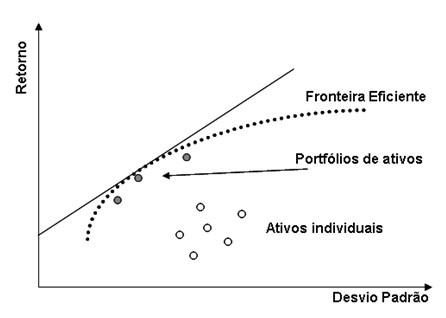
\includegraphics[height=4cm,keepaspectratio]{marko_02.png}
 \end{center}
 
\end{frame}


\begin{frame}{Minicaso}

\begin{itemize}
  \item IFN:  índice setor financeiro
  \item IMOB: índice do setor imobiliário
  \item ICON: índice de consumo
  \item IEE:  índice de energia
  \item INDX: índice da indústria
\end{itemize}

\end{frame}

\begin{frame}{Ativos  IBOVESPA}

\begin{center}
 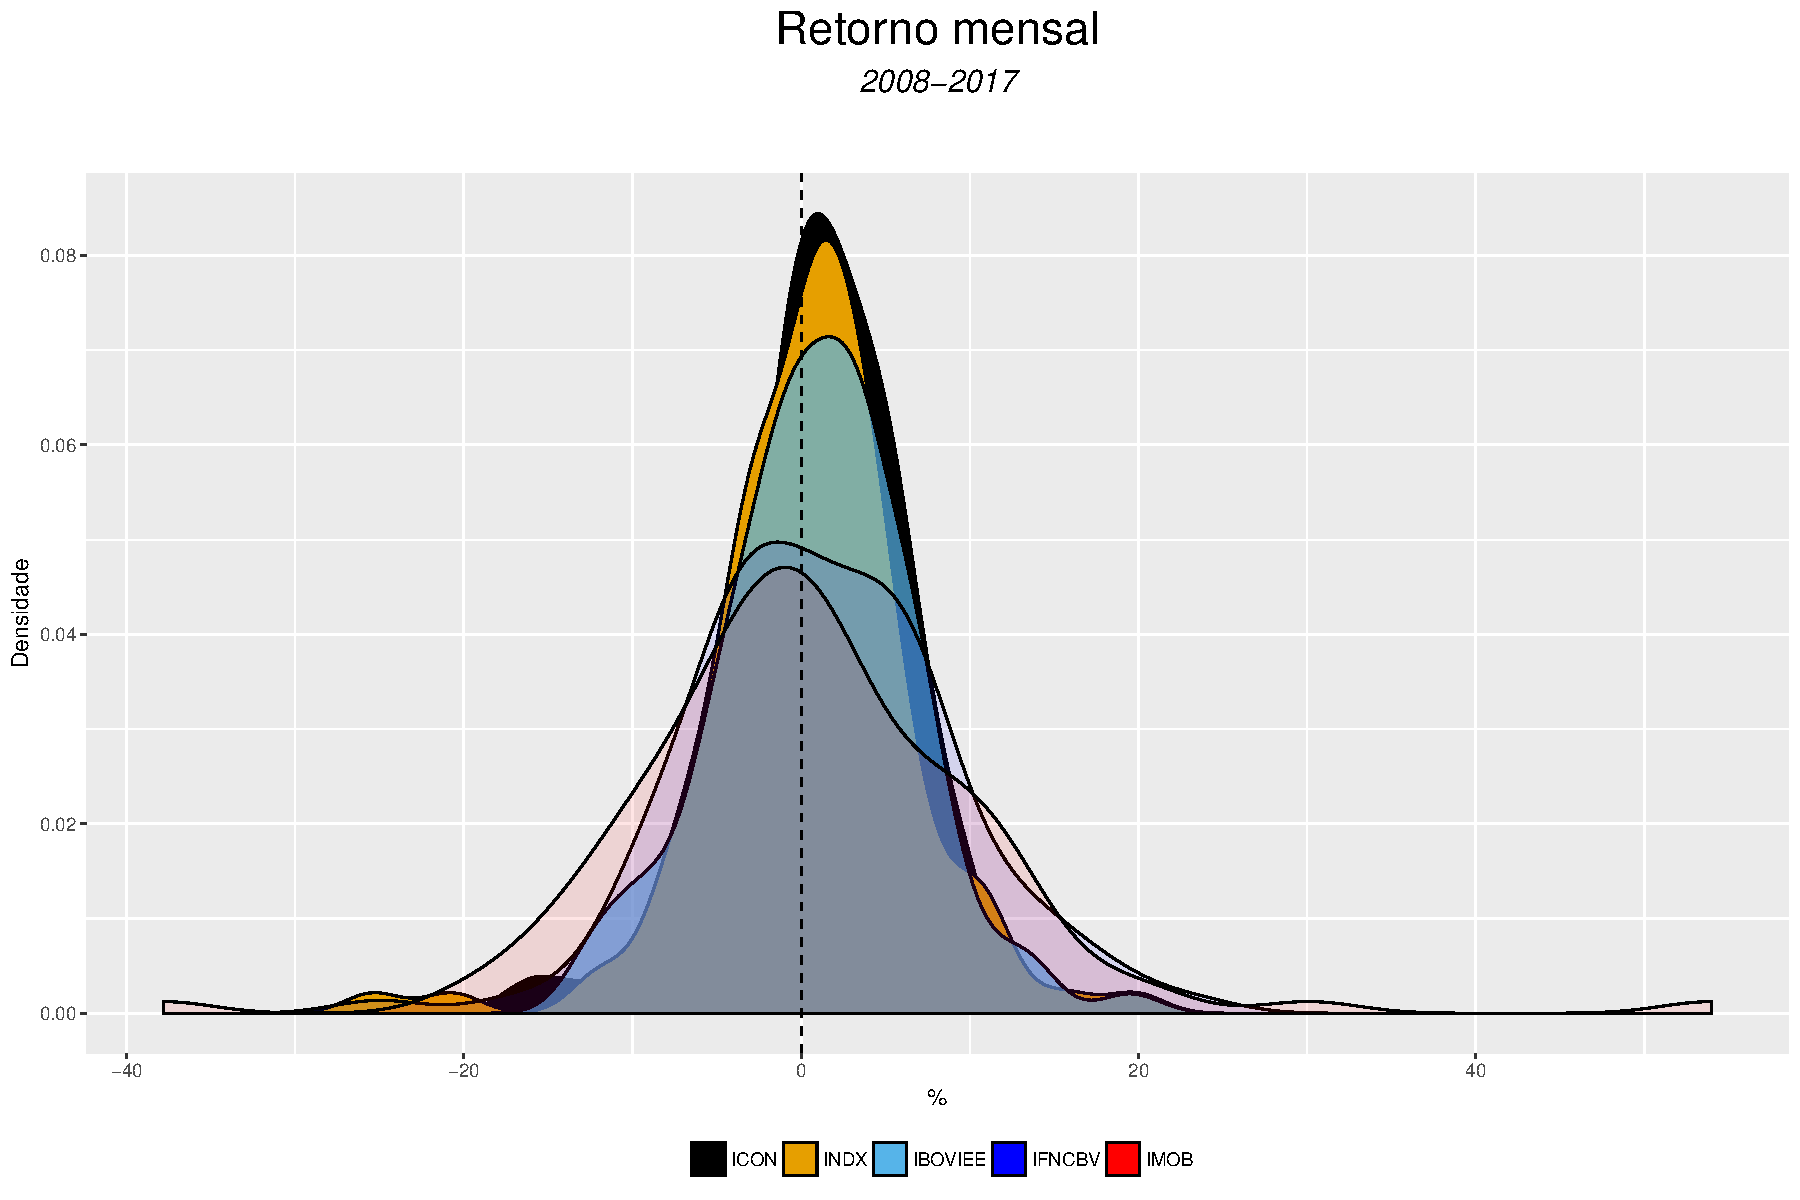
\includegraphics[height=8cm,keepaspectratio]{decritiva_indices.pdf}
 \end{center}


\end{frame}


\begin{frame}{Estatísticas}

% latex table generated in R 3.3.2 by xtable 1.8-2 package
% Sun Feb 18 11:14:16 2018
\begin{table}[ht]
\centering
\begin{tabular}{lrr}
  \hline
variable & M & DP \\ 
  \hline
ICON & 1.17 & 5.30 \\ 
  INDX & 0.50 & 6.14 \\ 
  IBOVIEE & 0.90 & 5.70 \\ 
  IFNCBV & 1.20 & 7.74 \\ 
  IMOB & 0.30 & 10.70 \\ 
   \hline
\end{tabular}
\end{table}


\end{frame}


\begin{frame}{Estatísticas}

\begin{center}
 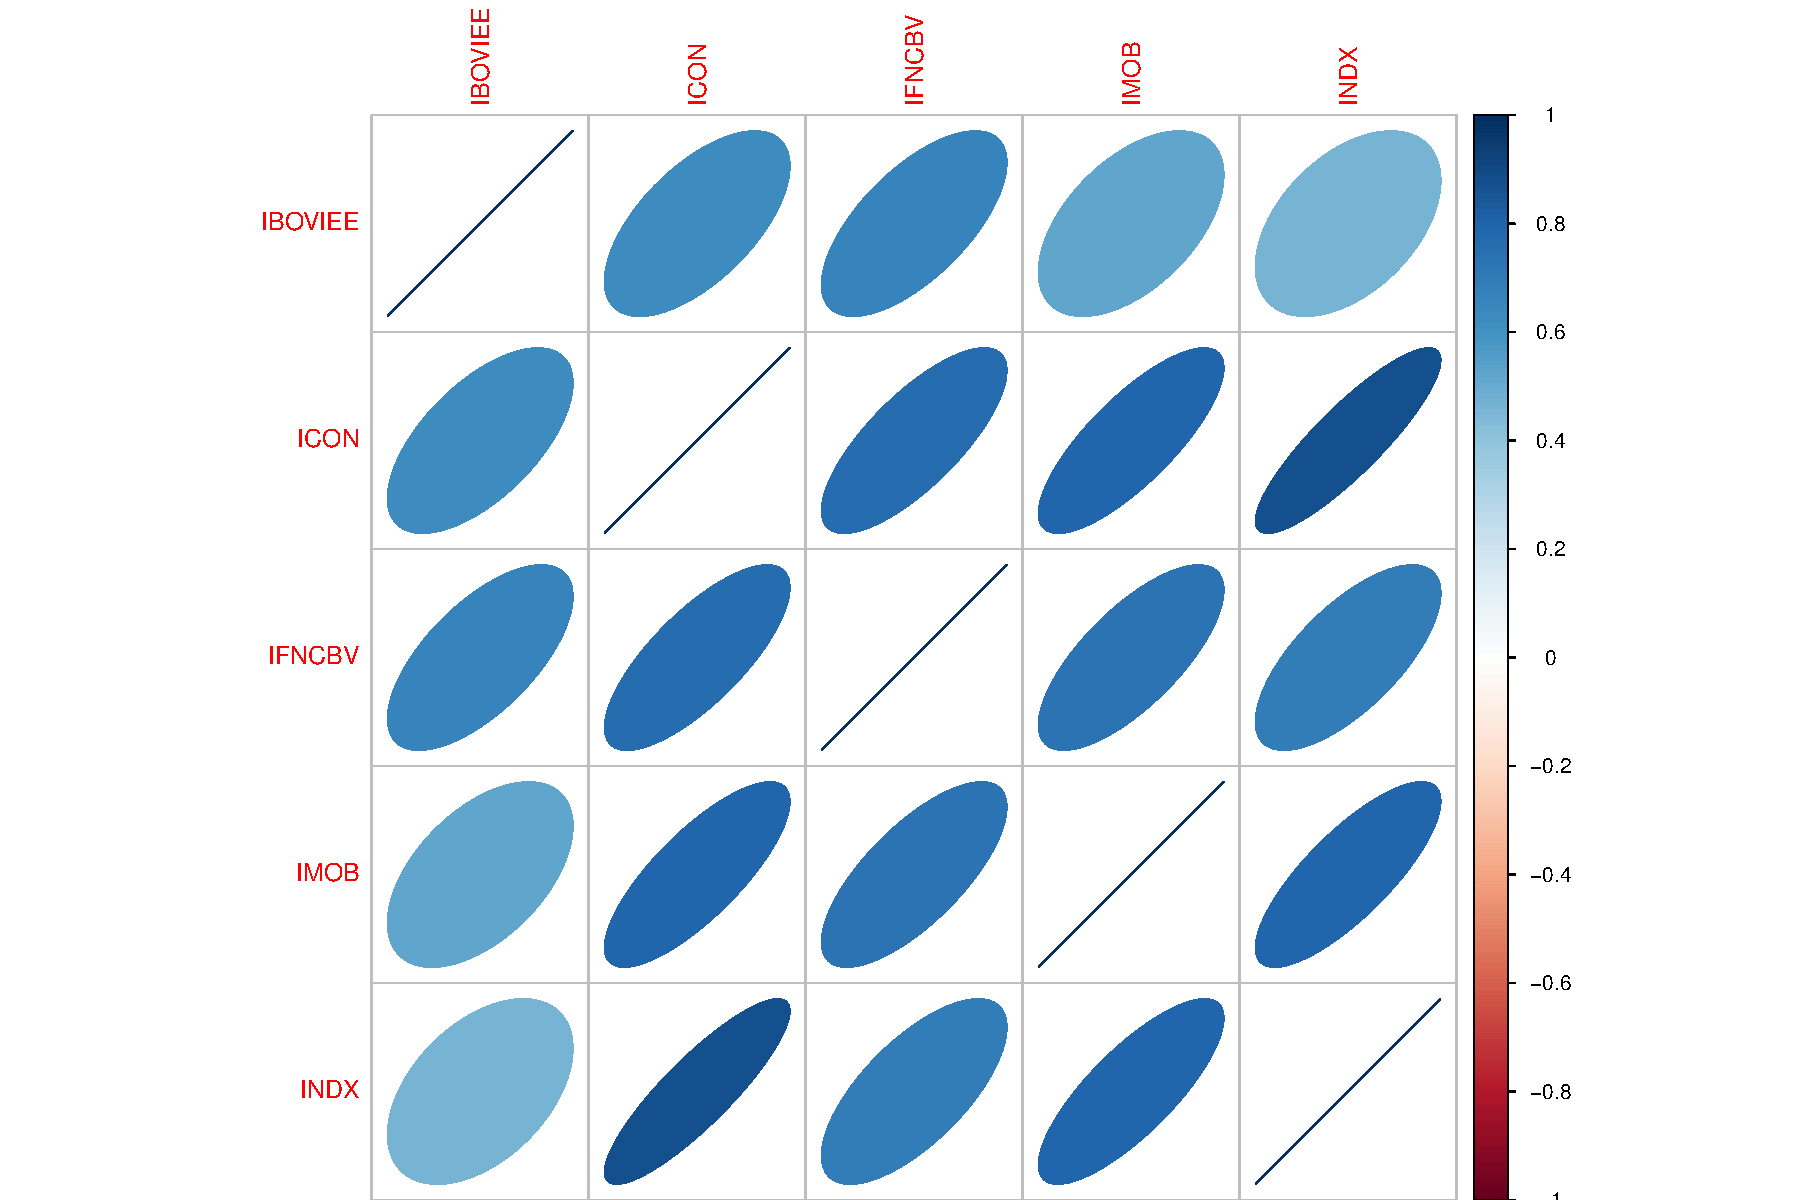
\includegraphics[height=8cm,keepaspectratio]{descritiva_cor.pdf}
 \end{center}


\end{frame}



\begin{frame}{Fronteira}

\begin{center}
 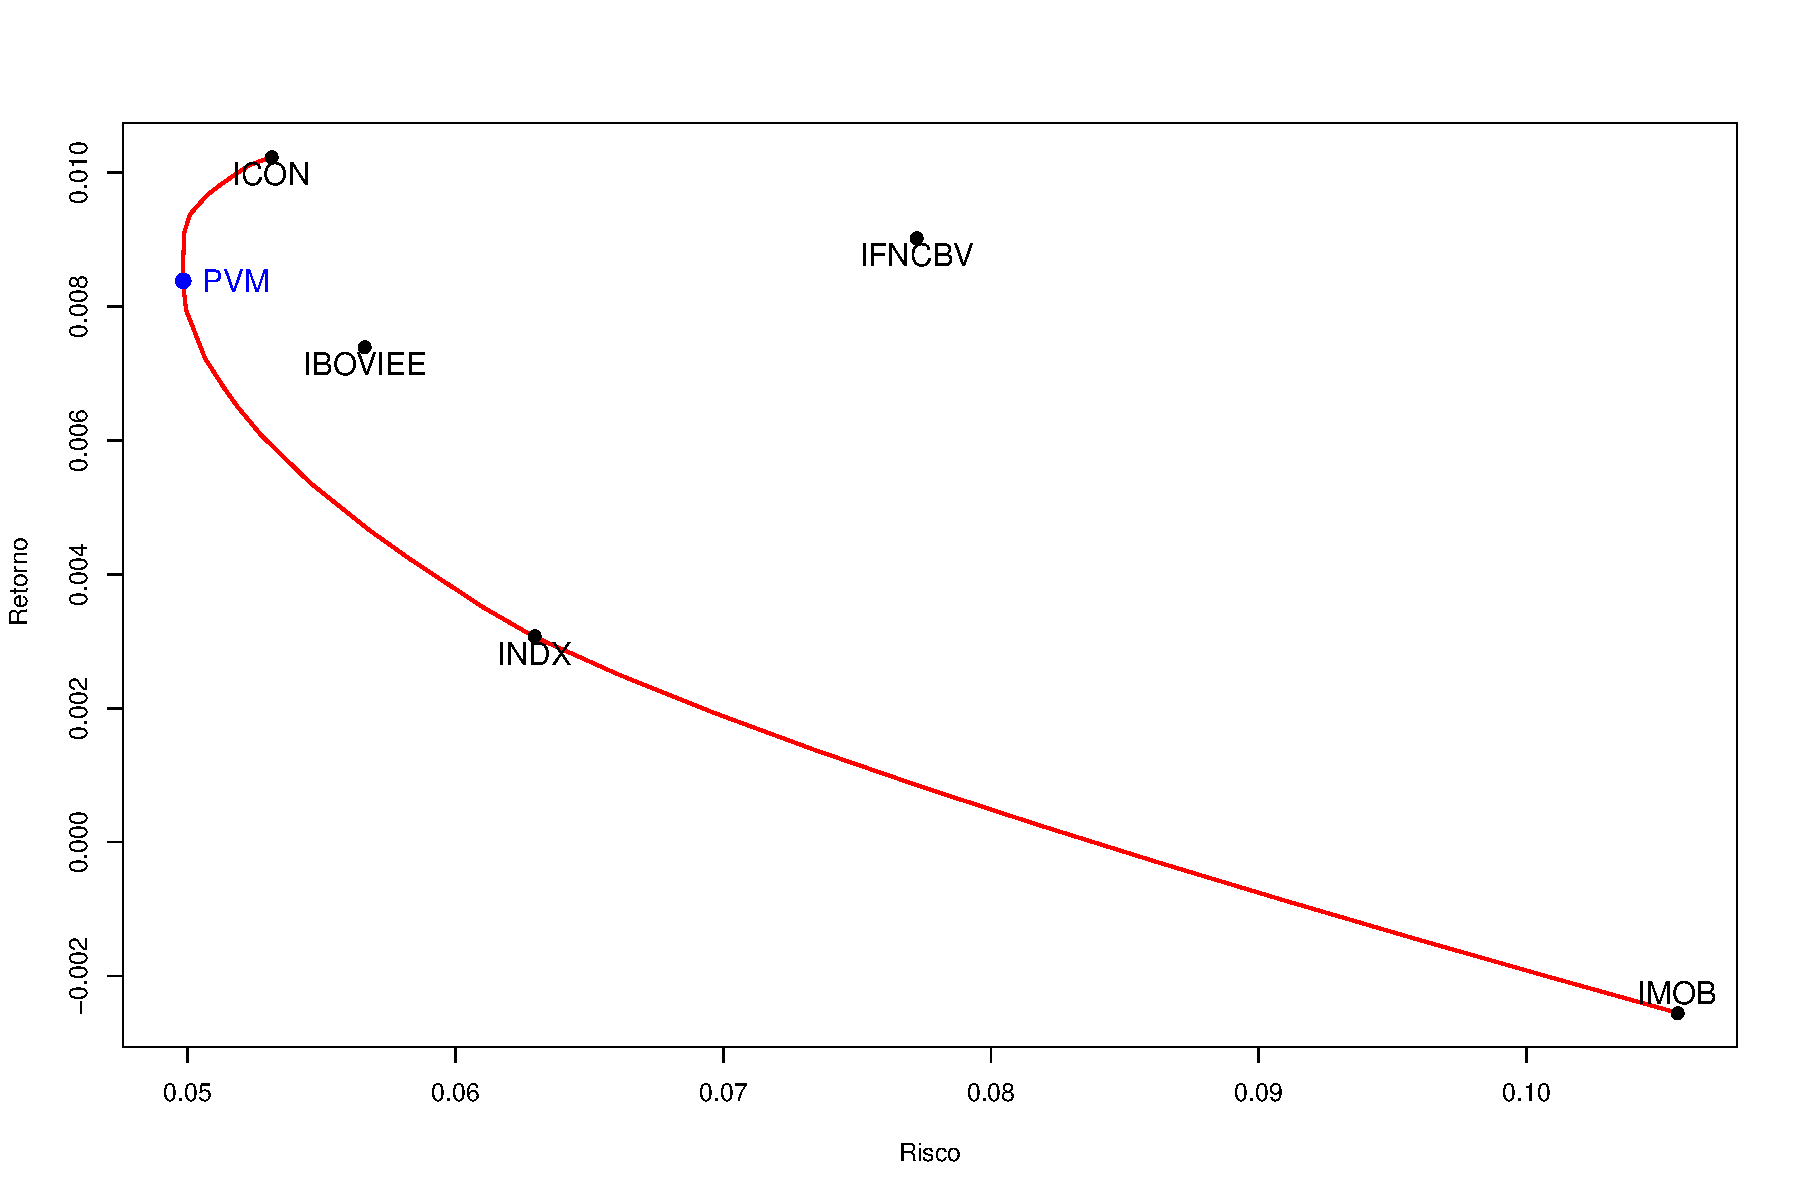
\includegraphics[height=8cm,keepaspectratio]{fronteira_ativos.pdf}
 \end{center}


\end{frame}


\begin{frame}{Série Temporal}

\begin{enumerate}
\item transversal
\item longitudinal
\end{enumerate}

\end{frame}

\begin{frame}{Objetivo}

Apresentar:

\begin{itemize}
\item Métodos numéricos para séries temporais 
\item Desenvolvimentos recentes
\item Principais aplicações
\end{itemize}

\end{frame}

\begin{frame}{Expectativa ao final}

\begin{itemize}
\item Identificar diferenças entre os principais métodos
\item Relacionar a aplicações em Finanças
\item Conhecer referências clássicas e recentes na área
\end{itemize}

\end{frame}



\section{Método}


\begin{frame}{Método}

\begin{enumerate}
\item Bootstrap
\item Monte Carlo
\item Markov Chain Monte Carlo
\end{enumerate}

\end{frame}

\subsection{Bootstrap}

\begin{frame}{Bootstrap}

O que é Bootstrap

\end{frame}


\begin{frame}{Sistemas Complexos}

Por que isso é interessante ?

\end{frame}


\subsection{Monte Carlo}

\begin{frame}{Monte Carlo}

História do Método Monte Carlo

\end{frame}


\begin{frame}{Monte Carlo}

Por que isso é interessante ?

\end{frame}

\subsection{Markov Chain Monte Carlo}

\begin{frame}{Markov Chain Monte Carlo}

O que é Markov Chain Monte Carlo?

\end{frame}


\begin{frame}{Markov Chain Monte Carlo}

Por que isso é interessante ?

\end{frame}




\section{Modelos}



\subsection{Modelos de Espaços de Estados}

\begin{frame}{Modelos de Espaços de Estado}

O que são modelos de espaços de estados

\end{frame}


\begin{frame}{Modelos de Espaços de Estado}

Por que isso é interessante ?

\end{frame}



\section{Filtro de Partículas}



\begin{frame}{Filtro de Partículas}

O que é Filtro de Partículas

\end{frame}



\begin{frame}{Série Temporal}


\begin{enumerate}

\item Complexidade (transversal)

\item  Complexidade (longitudinal)

\end{enumerate}

\end{frame}

\subsection{Aplicação}


\begin{frame}{Aplicações}

\begin{itemize}

\item Retorno

\item Volatilidade
\end{itemize}

\end{frame}


\begin{frame}{Retorno}

Modelo para retorno
\end{frame}


\begin{frame}{Volatilidade}
Modelo para volatilidade
\end{frame}





\subsection{Implementações}

\begin{frame}{Implmentação}

\begin{itemize}

\item R

\item Python


\end{itemize}

\end{frame}



\section{Considerações finais}
\begin{frame}{Considerações finais}

Flexibiliza

\end{frame}



\begin{frame}[allowframebreaks]%in case more than 1 slide needed
    {\tiny
    \bibliographystyle{apalike}
    \bibliography{bibli}
    }
\end{frame}

\end{document}



